\glsresetall

\section{Bringing the Dynamic Microbiome to Life with Animations}

\subsubsection{Abstract}

Our bodies and natural environment contain complex microbial communities, colloquially termed microbiomes. We previously created a web-based application, EMPeror, for visualizing ordinations derived from comparisons of these microbiome communities. We have now improved EMPeror to create interactive animations that connect successive samples to highlight patterns over time.

\subsection{Introduction}

Recent developments in high throughput DNA sequencing, improvements in molecular methods, and the continual increase in computational power have enabled microbiome researchers to test ever-more sophisticated hypotheses and study designs. Just a decade ago, a microbiome study with a few dozen samples was considered large. However, new technologies now enable studies with thousands of samples that can explore differences at the scale of population or environmentals.

One iconic result of these studies is the presentation of aggregated microbiomes from different human body sites within a single plot, where samples from equivalent body sites across many different individuals all cluster together (for an example, see Figure~\ref{anim_fig1}). This body site clustering was initially observed in a study of 9 people \cite{RN3738}, and then replicated across hundreds of people in the \gls{hmp} \cite{RN3752}. As useful as these static snapshots have been in examining the variation in diversity across populations, they do not reveal temporal dynamics, which may stem from intrinsic properties of the ecosystem such as inter-species interactions or external drivers such as drugs or diet (in humans) or envionmental perturbations. As seen in macroscopic ecology, changes in the relative abundance of organisms can occur on short time scales. Given that population doubling times of some bacteria can be less than 20 minutes, these time scales can be potentially very short for commensal communities. A single gram of stool can contain over one billion microbial cells, 1000 times the density of microbes in the ocean surface. These microbes are represented by hundreds of species, thousands of strains, and an estimated 3.3 million microbial genes \cite{RN4030}. Individual species and strains compete for resources (e.g., fiber), which can impose limitations on organism populations as the supply and demand of resources are dynamic overtime. Additionally, there are time-dependent bacteriophages which target and kill specific bacteria, or in some cases, promote \gls{hgt}, which can alter the strains (e.g., antibiotic resistance genes are commonly transferred via \gls{hgt}). Furthermore, many selective pressures act on the microbiome. For example, the human immune system acts as a regulatory force for the constituent organisms. This includes the innate and adaptive immune system, but also the variety of white blood cells and their antimicrobial glycoproteins. Additionally, microbial cells, many of which are capable of highly optimized metabolic processes, are subjected to a constantly changing set of compounds from the host's diet, as well as an intermittent exposure to antibiotics and other xenobiotics (in the case of diseased subjects, antibiotic use can lead to dysbiotic microbiomes, especially when taken frequently and at high doses).  

The emergence of quantitative microbial ecology dynamics will be important for strengthening our basic scientific understanding of the microbial world.  Additionally, it will also quickly become an essential tool for medicine. Currently, when antibiotics or other pharmaceuticals are given, the doctor does not know the “state” of the microbiome or how it will be altered. Being able to read out and predict changes in the microbiome will enable a field of precision medicine, for restoring the altered ecology to a healthy one. Similarly, there is great hope that designer pre- and probiotics will be powerful tools for `gardening' one's microbiome back to health.  However, until more quantitative and large-scale trials have been performed with longitudinal tracking of the changes in the microbiome ecology, the precise impact of these tools will remain, at best, a conjecture.

With the improved understanding of human microbial dynamics, the conceptual framework of medicine will continue to experience big changes. As recently described \cite{RN4020} many fundamental concepts from ecological theory are directly applicable to the host-microbiome ecology. However, these topics have not yet been widely incorporated as part of general medical training.  Concepts of succession and community assembly in previously unoccupied habitats (infant growth of microbial diversity), assembly after disturbance (recovery from antibiotics) and blooming of invasive species (food poisoning by pathogens).  Each of these topics will be elucidated in the coming decade by analyzing time series of microbial ecologies, especially in testings with defined perturbations, and integrated with metabolomics, metatranscriptomics, metaproteomics, and host biomarkers.

\subsection{Ordinations}
Datasets that have been obtained from DNA sequencing often have very high dimensionality, up to thousands of dimensions for each sample. Given the high dimensionality of  microbiome studies, the use of dimensionality reduction techniques, otherwise known as ordinations, have been widely used in the field (some examples include \gls{pca}, \gls{pcoa}, \gls{nmds}, and \gls{ca}). These techniques are analogous to modern photography: photographs capture 2D images of a 3D environment, and although they do not capture all of the information about the landscape, they can provide enough information to differentiate and identify objects.  Similarly, ordination methods are valuable tools for capturing snapshots of these microbial populations and better understanding the major driving factors affecting these populations. 

Although it is clear that the frontier of microbiome research is shifting to understanding microbiome dynamics, it remains a challenge to `see' the dynamics in these increasingly large datasets. Traditional time-series analysis techniques were developed around densely sampled and evenly collected variables, restrictions that are often impossible in clinical and ecological settings. Beyond these technical limitations with sampling, the complex dynamics of most microbial ecology datasets violate assumptions of periodicity and stationarity, used in many statistical methods for time-series analysis. For an expanded discussion and review of this topic, see \cite{RN4029}.

A few pioneering studies have been published for microbiome time series, but these visualizations were typically performed using custom `one-off' software that is generally harder to modify, maintain and reuse. However, these examples showed the promise of visualizing microbiome dynamics.  For instance \cite{RN4022}, described in detail the per-subject alpha and beta diversity variations, as well as the individual variability observed in the time point to time point comparisons. Another remarkable example presented by \cite{RN4021} examined pre- and post-dietary intervention comparisons at the microbiome and gene expression level. Similarly, \cite{RN4025} used the data from an infant's first 27 weeks of life to show that you can visualize the assembly of gut communities and contextualize it with the data of healthy human adults of the HMP\@. This analysis shows a step-by-step transition of the infant's communities as they transition into one of a healthy adult. \cite{RN4023} showcased the variability in the three body sites of the two surveyed subjects. More importantly, it gradually painted a picture, sample by sample, of the overall stability and dynamics present in the dataset. 

\subsection{EMPeror}
EMPeror is a response to the many requirements that are specifically relevant to high throughput microbiome studies.  The core idea behind this software is to allow users to rapidly explore a dataset, traversing hundreds of sample metadata categories and minimizing the necessity of custom plotting code. All of this can occur without requiring a complex software installation or domain-specific knowledge.

EMPeror \cite{RN3814} is a web-enabled scatter plot viewer for microbiome analysis that was originally made available in 2013 as part of the QIIME pipeline \cite{RN110}, and developed for the Earth Microbiome Project\footnote{\url{http://www.earthmicrobiome.org}}. To use EMPeror, two files need to be provided, the first and most important is the sample metadata file, which contains covariate information about each sample, and the second file is a matrix specifying coordinate positions for each sample along a set of axes. In general, for microbiome studies, the coordinate positions are derived using \gls{pcoa}. Besides allowing the easy exploration of high dimensional color ordination spaces (such as \gls{pca} or \gls{pcoa}), EMPeror supports more specialized techniques, ranging from displaying jackknifed-resampled data to assess statistical confidence in clustering, to displaying procrustes analysis plots to determine the goodness of fit between two independent datatypes, and even being able to visualize biplots. As of version 0.9.5, users can now create animations inside the user interface without the necessity of any additional computation.

Like most functionality in EMPeror, animations themselves are made possible by selecting two metadata categories, a \textit{trajectory} category and a \textit{gradient} category. The first category determines how the samples are grouped together (e.g.\ individual), and the second category describes the order of the grouped samples. As readers might suspect, the ordering is only unambiguous when the values in the \textit{gradient category} are numeric; therefore, we recommend that only these data types are used. Along with these metadata selectors, EMPeror displays a \textit{play}, a \textit{pause}, and a \textit{rewind} button. These control the state of the traces being presented on screen.

With this mapping, samples that belong to the same \textit{trajectory} are subsequently connected by an animated trace (sample by sample). The traces are created by linearly interpolating a series of points between two samples. The number of points present in this interpolation depends on the absolute difference between the two samples in the \textit{gradient}, meaning that samples that were collected further apart along a gradient (e.g., if some samples are daily and some are weekly) will take longer to be connected in the animation than samples that were collected closer in the \textit{gradient}. This allows heterogeneous sampling schemes, common in clinical trials or when some samples are lost or destroyed during processing, to be accommodated in the same animation.

Importantly, these animations do not interfere with the interactivity of a plot. The rest of the controllers (used to manipulate the rotation, zooming, coloring, size, opacity, etc.) remain available and can be used interactively to create a narrative that is more relevant for the data. Lastly, EMPeror is a stand-alone application, that can be easily integrated into a software workflow, for instance using Jupyter notebooks \cite{RN162}.

\subsection{Example}
To showcase the utility of this particular type of visualization, we will reproduce the supplementary video presented in 2015 \cite{RN4026}, where four \gls{cdi} patients are surveyed before and after a \gls{fmt} to ameliorate the consequences of this enteric infection.

To create  this visualization, we must combine this indiviual dataset with the 16S rRNA amplicon samples from the \gls{hmp} \cite{RN3752}, which includes thousands of microbiome samples collected from 242 healthy individuals. These HMP samples create a visual `map' of normal oral, skin, vagina, and stool microbiomes and provide context for the \gls{cdi} samples. To combine these studies, we used  Qiita\footnote{\url{https://qiita.ucsd.edu}}, an open-source platform for analysis and visualization of microbiome datasets. Qiita allows users to combine samples, perform the necessary computations for \gls{pcoa} (among other analyses), and allows for visualizing the result in EMPeror. 

For this example, we selected the number of days since the \gls{fmt} procedure as the \textit{gradient} category and we selected the subject as the \textit{trajectory} category. By animating these traces, we first observe that the original patients with \gls{cdi} had gut microbiomes that did not resemble healthy adult fecal communities. Immediately after the \gls{fmt}, we observe a rapid transition into a health state, which can be inferred from the movement of the sample locations by the end of the trajectory to the normal stool region defined by the \gls{hmp} (Figure~\ref{anim_fig1}). Critically, these transitions were associated with the patient's immediate recovery from the illness.

\begin{figure}[htbp]
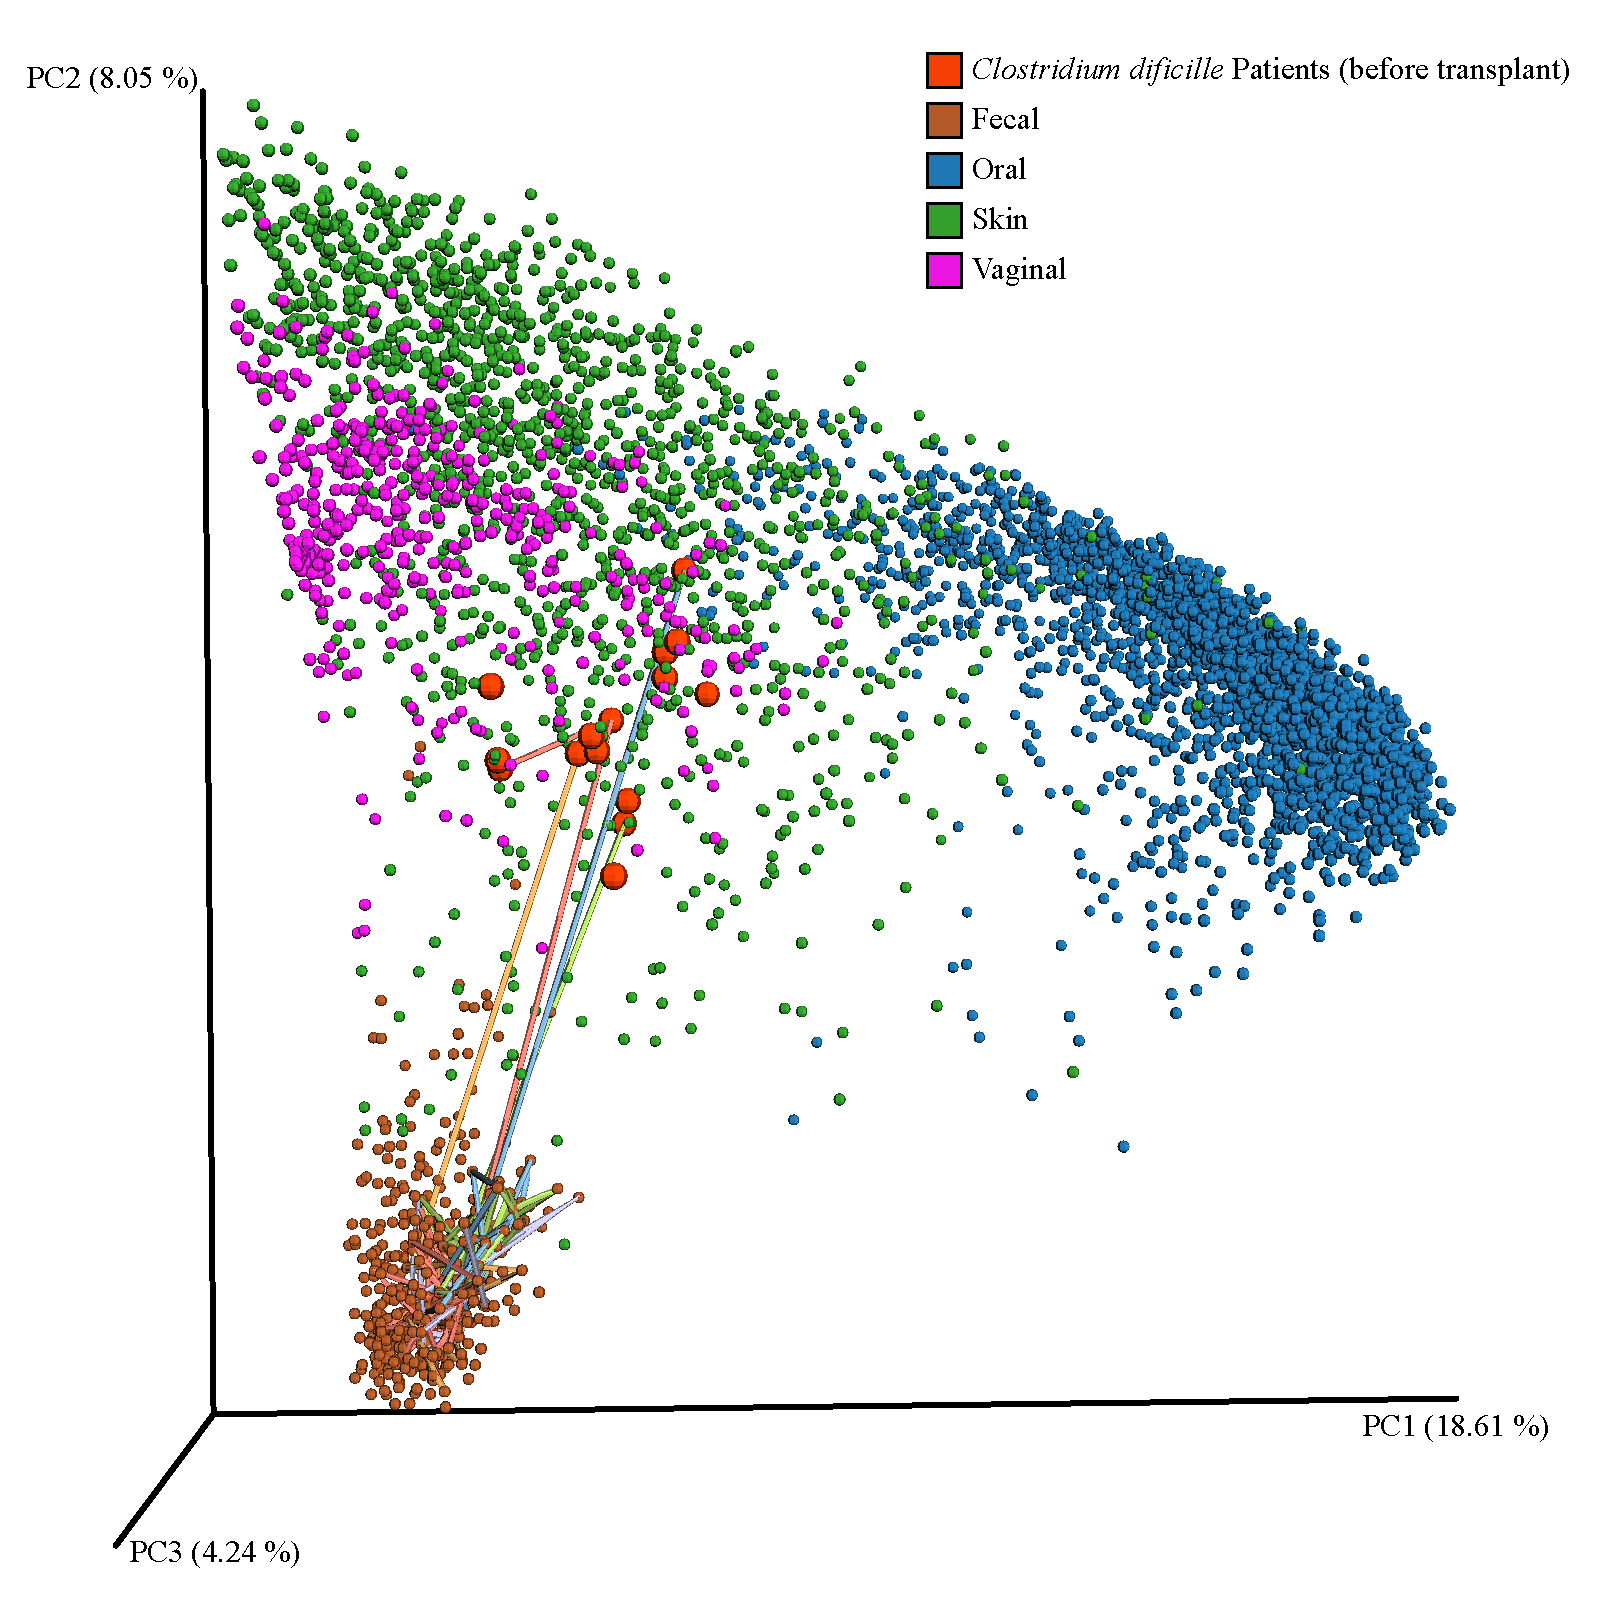
\includegraphics[width=\columnwidth]{animations-figures/figure1}
\caption[Case study: remission of Clostridium difficile Infection]{\textbf{Case study: remission of Clostridium difficile Infection.} \textit{Principal Coordinates Analysis Plot of unweighted UniFrac distances.} After receiving the fecal transplant, the patients undergo a dramatic transition in their gut microbiomes. Samples from healthy individuals are colored: blue for oral, green for skin, pink for vaginal and brown for fecal communities. Patient samples (preceding the transplant) are colored in orange, the traces indicate the trajectory they follow over time (only four subjects receive a transplant). Access this interactive animation using your web browser: \url{http://emperor.microbio.me/animation/}}
\label{anim_fig1}
\end{figure}

\subsection{Limitations}
The objective of ordinations is to find the dimensions that best describe as much as possible the variation in a dataset, and therefore reduce the amount of information that we have to interpret. This property is most often useful for its ability to distinguish between groups of samples. However, it also makes this technique sensible to outliers. Consequently, it is important to remember that the variation explained in a statistical model does not necessarily correspond to biological importance. In fact, some methods of measuring distance between samples and ordination techniques for reducing dimensionality can explain much of the variation in a given dataset, but fail to reveal biologically important patterns \cite{RN3802}. In addition, \gls{pcoa} is susceptible to an artifact called the horseshoe effect, where the shared absence of taxa in the middle of the gradient cause the ends to appear similar and wrap around (other techniques such as Non-metric Multidimensional Scaling are susceptible to a related problem called the arch effect, where the second axis is a distorted reflection of the first), and very sparse data matrices where most samples are highly dissimilar to one another can produce artifacts resembling spikes at 90 degree angles to one another, Consequently, choosing the wrong distance metric or dimensionality reduction method for a dataset can result in visual artifacts that render those visualizations unusable. These problems are less frequent, but still possible, when phylogenetic distance metrics such as UniFrac \cite{RN133} are used.
Animating the transitions between samples provides a useful visual aid. However, the observed patterns of variation still need to be asessed using descriptive statistics. Differences among sets of community samples can be assessed using the \gls{anosim} or a \gls{permanova}. These statistical tests compare the groups using the distance matrix to provide a statistic that measures whether sample category labels tend to group similar samples together more often than a random shuffling of the labels. Alternatively, feature-level differences can be assessed using compositional analyses, correlation networks or discriminant features between two groups (using supervised and unsupervised machine learning techniques). 

In our experience, the interpretability of animated ordinations is most commonly affected in two cases. The first case can be observed when an inappropriate frame of reference is used, or when only the animated traces are presented. For the example above, the HMP data provides a relevant context due to the types of samples being characterized and the size of the study. However, a reference frame that included only oral samples, or that contained only a single stool sample, would not provide nearly as relevant a data frame for display, and the resulting animations would be difficult to interpret. The second case occurs when many trajectories are animated simultaneously, making the ordination busy and increasing the difficulty of correctly identifying the patterns of variation that are most biologically relevant. This limitation can be overcome by choosing more similar sets of samples to display, such as patients with more consistently defined clinical phenotypes.

\subsection{Conclusions}
Microbiome studies are steadily increasing in size and complexity, challenging our ability to unravel the structure of the ecological interactions occurring at the  microbial scale. As researchers, the software we use greatly impacts our ability to ask questions of the data. Platforms like the Jupyter Notebook have greatly facilitated reproducibility of analyses.  The success of the Notebook has been in part, due to building on top of an open and common web infrastructure, the same that Emperor has adopted. Interactive animations like the example presented above, can be directly shared with anyone that has access to a modern web browser, whether it be in a personal computer or in a mobile device.

Sample information (also known as sample metadata) is indispensable to data reuse and necessary for the creation of complex visuals, like in Figure 1. This task was partly possible by leveraging the standardization of sample metadata enforced in Qiita. Without standardization, future generations must undertake the burden of post-hoc metadata curation, a process that is deeply frustrating and impossible to automate.

Finally, although EMPeror provides a handful of ways to interrogate a dataset, we urge the community to create other open source interactive tools that democratize robust, reproducible and interactive analysis techniques. These tools should not be usable by only a few experts, but instead must target broader audiences that can benefit from these technological advances.

\subsection{Availability}
The source code and documentation for version 0.9.60 can be found online\footnote{\url{http://biocore.github.io/emperor/}}. Additionally a tutorial (including the data) to generate Figure~\ref{anim_fig1} can also be found online\footnote{\url{http://biocore.github.io/emperor/build/html/tutorials/animations.html}}. 

